\documentclass[12pt]{article}
\usepackage[top=1in, bottom=1in, left=.75in, right=.75in]{geometry}

\usepackage{amsmath}
\usepackage{fancyhdr}
\usepackage{graphicx}
\usepackage{txfonts}
\usepackage{multicol}
\usepackage{wrapfig}
\usepackage[scaled=0.86]{helvet}
\renewcommand{\emph}[1]{\textsf{\textbf{#1}}}
\usepackage{anyfontsize}
% \usepackage{times}
% \usepackage[lf]{MinionPro}

%%TIKZ
\usepackage{tikz,pgfplots}
\usetikzlibrary{calc}
\usetikzlibrary{shapes}
%\pgfplotsset{my style/.append style={axis x line=middle, axis y line=middle, xlabel={$x$}, ylabel={$y$}, axis equal }}
%OTHER
%\pgfplotsset{my style/.append style={axis x line=middle, axis y line=middle, xlabel={}, ylabel={}}}

\pgfplotsset{my style/.append style={axis x line=middle, axis y line=middle, 
xlabel=$x$,ylabel=$y$,
every axis x label/.style={
    at={(ticklabel* cs:1)},
    anchor=west,
},
every axis y label/.style={
    at={(ticklabel* cs:1)},
    anchor=south,
},}}

\def\degC{{}^\circ{\rm C}}
\def\ra{\rightarrow}

\newcommand*\circled[1]{\tikz[baseline=(char.base)]{
            \node[shape=ellipse,draw,inner sep=2pt] (char) {#1};}}

\newcommand{\blank}[1]{\rule{#1}{0.75pt}}

\parindent 0pt
\parskip 4pt
\pagestyle{fancy}
\fancyfoot[C]{\emph{\thepage}}
\fancyhead[L]{\ifnum \value{page} > 1\relax\emph{Math 251: Midterm 2}\fi}
\fancyhead[R]{\ifnum \value{page} > 1\relax\emph{7 April 2020}\fi}
\headheight 15pt
\renewcommand{\headrulewidth}{0pt}
\renewcommand{\footrulewidth}{0pt}
\let\ds\displaystyle
\def\continued{{\emph {Continued....}}}
\def\continuing{{\emph {Problem \arabic{probcount} continued....}}\par\vskip 4pt}

\newcounter{probcount}
\newcounter{subprobcount}
\newcommand{\thesubproblem}{\emph{\alph{subprobcount}.}}

\def\problem#1{\setcounter{subprobcount}{0}%
\addtocounter{probcount}{1}{\emph{\arabic{probcount}.\hskip 1em(#1)}}\par}

\def\ecproblem#1{{\emph{Extra Credit. \hskip 1em(#1)}}\par}

\def\subproblem#1{\par\hangindent=1em\hangafter=0{%
\addtocounter{subprobcount}{1}\thesubproblem\emph{#1}\hskip 1em}}

\def\probskip{\vskip 10pt}
\def\medprobskip{\vskip 2in}
\def\subprobskip{\vskip 45pt}
\def\bigprobskip{\vskip 4in}


\begin{document}
{\emph{\fontsize{26}{28}\selectfont Math F251\hfill
{\fontsize{32}{36}\selectfont Midterm 2}
\hfill Spring 2020}}
\vskip 1cm
\strut\vtop{\halign{\emph#\hskip 0.5em\hfil&#\hbox to 2in{\hrulefill}\cr
\emph{\fontsize{18}{22}\selectfont Name:}&\cr}}
\hfill
\vtop{\halign{\emph{\fontsize{18}{22}\selectfont #}\hfil& \emph{\fontsize{18}{22}\selectfont\hskip 0.5ex $\square$ #}\hfil\cr
Section: & F01 (Faudree)\cr
\noalign{\vskip 4pt}
         & F02 (Bueler)\cr
\noalign{\vskip 4pt}
         & UX1 (Van Spronsen)\cr}}

\vskip 2cm
{\fontsize{18}{22}\selectfont\emph{All students must affirm the following statements by initialing in the blanks provided. Students using their own paper must write out the statements in full.}}

\underline{\hspace{1in}} I will not seek or accept help from anyone.  

\underline{\hspace{1in}} I will not use a calculator, books, notes, the internet or other aids.

\underline{\hspace{1in}} I understand that answers without work will not be awarded credit.


Good luck!

\vskip 1cm
\def\emptybox{\hbox to 2em{\vrule height 16pt depth 8pt width 0pt\hfil}}
\def\tline{\noalign{\hrule}}
\centerline{\vbox{\offinterlineskip
{
\bf\sf\fontsize{18pt}{22pt}\selectfont
\hrule
\halign{
\vrule#&\strut\quad\hfil#\hfil\quad&\vrule#&\quad\hfil#\hfil\quad
&\vrule#&\quad\hfil#\hfil\quad&\vrule#\cr
height 3pt&\omit&&\omit&&\omit&\cr
&Problem&&Possible&&Score&\cr\tline
height 3pt&\omit&&\omit&&\omit&\cr
&1&& 10 &&\emptybox&\cr\tline
&2&& 10&&\emptybox&\cr\tline
&3&& 10&&\emptybox&\cr\tline
&4&& 8 &&\emptybox&\cr\tline
&5&& 12&&\emptybox&\cr\tline
&6&& 6 &&\emptybox&\cr\tline
&7&& 12 &&\emptybox&\cr\tline
&8&& 10 &&\emptybox&\cr\tline
&9&&  10&&\emptybox&\cr\tline
&10&& 12 &&\emptybox&\cr\tline
&Total&&100 &&\emptybox&\cr
}\hrule}}}


\newpage
\vspace*{-0.3in}



%Problem 1, Section 3.4 like #63

\problem{10 points} A table of values for $f(x),\: g(x),\: f'(x)$ and $g'(x)$ is given.

\begin{center} 
\begin{tabular}{|c||c|c||c|c|}
\hline
$x$&$f(x)$&$f'(x)$&$g(x)$&$g'(x)$\\
\hline \hline
1&3&1&2&8\\
\hline
2&4&3&2&4\\
\hline
3&5&2&1&6\\
\hline
\end{tabular}
\end{center}
\subproblem{} If $h(x)=x^2f(x) -g(x),$ find $h'(3).$
\vfill
\subproblem{} If $h(x)=f(g(x)),$ find $h'(1).$
\vfill

%: PROBLEM 2 Section 3.7 and 3.8 Exponential growth or decay *Jill
%{Section 3.7 \#7} 
\problem{10 points}  A particle moves on a vertical line so that its coordinate $y$ at time $t$ is $y=t^4-3t^2+2,$ where $t\geq 0.$
\subproblem{} What is the initial position of the particle? \vfill
\subproblem{} When is the particle moving downward? \vfill
%\subproblem{} At $t=1,$ is the particle speeding up or slowing down? Explain your answer.
\vfill
\newpage

%Problem 3
%Section 3.8 \#3}  *Jill
\problem{10 points} On March 21, the Alaska Department of Health and Social Services finds 21 Alaskans are infected with a new virus. By March 31, the number of Alaskans infected has risen to 133.  Assume that the number of people infected grows at a rate proportional to the size of the infected population. %\textbf{Note:} Because you are not using a calculator, your answers here may not be nice simple numbers, like integers or rational numbers. That's ok. Complicated expressions like $\:\ln(2) + \sqrt{5}\:$ are fine.
\subproblem{} Write an equation that says that the number of people infected grows at a rate proportional to the size of the infected population.
\vfill
\subproblem{} Assuming the growth rate continues, with no mitigating factors, find an expression for the number, $N$, of Alaskans infected over time $t$ in days. \vfill
%\subproblem{} According to this model, how long does it take until 2100 Alaskans are infected? (Give units with your answer.) \vfill

%Problem 6, Section 4.1 Max/min. *Jill
% \textcolor{red}{Section 4.1 \#11} 
 \problem{8 points} Sketch a graph $f$ with domain $[1,4]$ such that $f$ has an absolute minimum but no absolute maximum. \vfill

 
%  %Problem 5, Section 3.10 Linear Approximations. *Hillary
%  \problem{8 points} 
% \subproblem{} Find the linearization of $f(x) = x^4$ at $x=2$. \vfill
% \subproblem{} Use your result in part (a) to approximate $(2.001)^4$.  \vfill
 
 \newpage
 
 %Problem 4, Section 3.9 Related Rates. *Hillary
 
 \problem{12 points} A ship passes a lighthouse at 3:30pm, sailing to the east at 5 mph, while another ship sailing due south at 6 mph passes the same point half an hour later.  How fast will the distance between the ships be increasing at 5:30pm? \vfill
 
 
 
  % section 4.5 type problem, includes L'Hopital's rule for horizontal asymptote
\problem{6 points}  Does the graph of the function $\displaystyle f(x) = \frac{3 \ln x}{1-x}$ have a vertical asymptote at $x=1$? Justify your answer using an appropriate limit.
\vspace{2in}

\newpage
%%Problem 7
%%\textcolor{red}{Section 4.1 \#47-62} *Jill
%\problem{XX points}  Let $f(x)=(x^2-9)^{2/3}.$
%\subproblem{} Find the critical numbers of $f(x).$ \vfill
%\subproblem{} Explain why $f(x)$ is guaranteed to have both an absolute minimum and an absolute maximum on the interval $[-1,2].$ \vfill
%\subproblem{} Find the absolute maximum and absolute minimum of $f(x)$ on $[-1,2].$ \vfill
%
 
 \problem{12 points} The graph of the \textit{\textbf{derivative}} $f'$ of a continuous function $f$ is shown. 

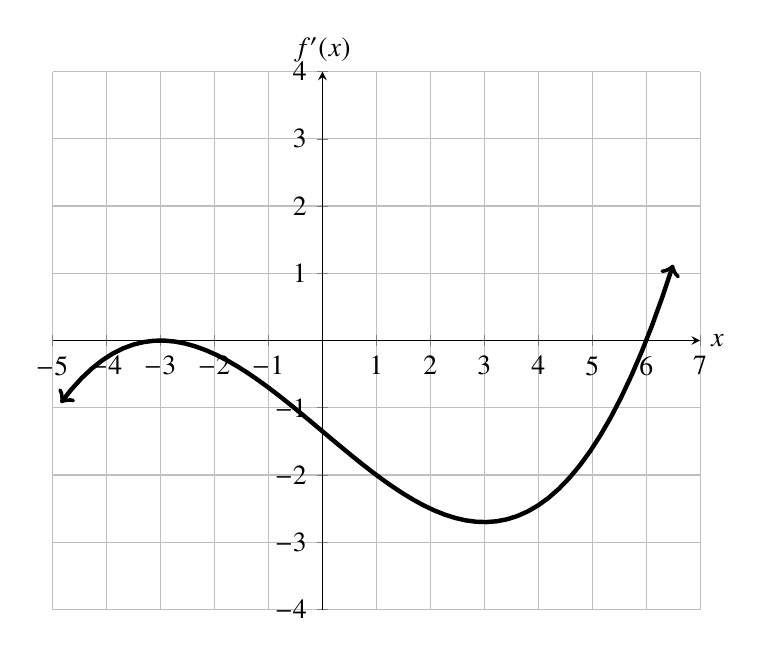
\begin{tikzpicture}
\begin{axis}[scale=1.2, my style, xtick={-5,-4,...,7}, ytick={-4,-3,...,4},
xmin=-5, xmax=7, ymin=-4, ymax=4, minor y tick num=0,
minor x tick num=0, mark size=5.0pt,
grid=both, ylabel=$f'(x)$,samples=60]
%\addplot[smooth, ultra thick, <->] coordinates {(-4.8,-0.8)(-4,-.2)(-3,0)(-2,-.2) (0,-1.3)(1.5,-2)(2,-1.8)(3,0) (4,1.6)(5,2)(6.5,2.5)};
\addplot[domain=-4.85:6.5, <->, ultra thick] {(x+3)^2*(x-6)/40};
% \addplot[only marks, mark size=2pt] coordinates {(0,-1.8) (7,2.4)};
\end{axis}
\end{tikzpicture}

\subproblem{} Determine the critical points of $f(x).$\\
\vfill
\subproblem{} At what values of $x$, does $f$ have a local maximum? Local minimum? Explain your answer.
\vfill
%\subproblem{} On what intervals is $f$ increasing or decreasing? Use interval notation.\\
%\vfill
%\subproblem{} At what values of $x$ does $f$ have a local maximum or minimum?\\
%\vfill
\subproblem{} On what intervals is $f$ concave upward? Concave downward? Use interval notation.\\
\vfill
%Or just 3 of these!
\newpage

%% 4.4 exercise #16, and a problem like example 6
%\problem{5 points}  Does the graph of   $f(x)= \frac{x^2}{1-\cos x}$ have a vertical asymptote at $x=0$? Justify your answer with a limit.

\vfill

\newpage
 


%\subproblem{} Determine the domain of $f$, and find the $x$- and $y$-intercepts.
%\vfill
\problem{10 points} A function and its first and second derivatives are given below.
$$f(x)=x^{5/3}-5x^{2/3}, \quad \quad f'(x)=\frac{5x-10}{3x^{1/3}}, \quad \quad f''(x)=\frac{10x+10}{9x^{4/3}}$$
\subproblem{} Find the intervals of increase and decrease, and identify the locations of any local maximum or minimum values.
\vfill
\subproblem{} Find the intervals of concavity and the $x$-values of any inflection points.
\vfill
%\subproblem{} Sketch the graph $y=f(x)$ on the given axes.
%
%\hfill \begin{tikzpicture}[scale=1.0]
%\draw [help lines,dashed] (-6.2,-3.2) grid (6.2,4.2);
%\draw [thick, ->] (-6.2,0)--(6.2,0) node[right] {$x$};
%\draw [thick, ->] (0,-3.2)--(0,4.2) node[above] {$y$};
%%\foreach \i in {-4,-2,2,4}
%%   {  \node[below] at (\i,0) {$\i$};  }
%%\foreach \i in {-2,2,4}
%%   {  \node[left] at (0,\i) {$\i$};  }
%\end{tikzpicture}

 \problem{10 points}  Sketch a graph that satisfies all of the conditions:
\begin{align*}
  &\text{domain } f = (-\infty,\infty), \hspace{5.0in}\\
  &f(3)=-1, \quad f'(3)=0  \\
  & f'(x)<0 \text{ when } x<3,f'(x)>0 \text{ when } x > 3,  \\
  &f''(x)<0 \text{ when } x<0, \quad f''(x)>0 \text{ when } x>0 \\
  &\displaystyle{\lim_{x \to -\infty} f(x)=4}\\
\end{align*}

\vspace{-40mm}

\hfill \begin{tikzpicture}
\begin{axis}[scale = 1.4, axis x line=middle, axis y line=
middle, xlabel={$x$}, ylabel={$y$}, xtick={-3,-2,-1,0,1,2,3,4,5,6}, ytick={-3,-2,-1,0,1,2,3,4}, xmin=-4, xmax=7, ymin=-4, ymax=5]
\end{axis}
\end{tikzpicture}

\newpage

 

 
 
 
 \problem{12 points}  The graph of the function $\displaystyle f(x) = \sqrt{\frac{x}{2}+1}$ is shown.

\begin{tikzpicture}[scale=1.0]
\begin{axis}[scale=1.0, axis equal, my style,
xtick={-2,-1,...,3}, ytick={0,1,...,3},
xmin=-2.5, xmax=3.5, ymin=0, ymax=2.2,
minor y tick num=1, minor x tick num=1,
samples=200]
%
\addplot[domain=-2:4,-,thick] {sqrt(0.5*x+1)};
\end{axis}
\end{tikzpicture}

\subproblem{}  Let $G(x)$ be the square of the distance from the origin to a point on the graph of $y=f(x)$.  Write an expression for $G(x)$.

\vfill
\subproblem{}  Use the expression for $G(x)$ to find the closest point on the graph $y=f(x)$ to the origin.

\vfill
\subproblem{}  Show your result by adding a point, with coordinates, to the graph.

\bigskip


 
 
 
 

\end{document}
%%%%%%%%%%%%%%%%%%%%%%%%%%
%%%%%%%END
%%%%%%%%%%%%%%%%%%%%%%%%%%


 